\documentclass[preprint,12pt]{elsarticle}
\usepackage{lineno}
\usepackage{graphicx}
\usepackage{amsmath,amssymb}
\usepackage{hyperref}
\usepackage{booktabs}
\usepackage[expansion=false]{microtype}
\modulolinenumbers[5]

\begin{document}

\begin{frontmatter}

\title{A Mislabeled Contrast, Recovered: Diagnosing and Correcting an Encode/Test-Phase Confound in Blocked EEG Decoding}

\author[inst1]{Muhammad Hassan Siddiqui\corref{cor1}\fnref{orcid1}}
\ead{hassansiddiqui0946@gmail.com}
\author[inst1]{Muhammad Adil Usmani\fnref{orcid2}}
\cortext[cor1]{Corresponding author.}
\fntext[orcid1]{ORCID (M.H.S.): 0009-0006-7271-9788}
\fntext[orcid2]{ORCID (M.A.U.): 0009-0004-2856-3419}
\affiliation[inst1]{organization={Independent Researcher},
                    city={Lahore},
                    country={Pakistan}}

\begin{abstract}
A label-dictionary error in our own analysis pipeline produced an original headline accuracy of 70.78\% for a Search-vs-Memorize EEG decoding contrast. This error belongs to our own analysis pipeline, not to the public dataset it was applied to. Each class label conflated four structurally distinct marker types, so that 75\% of each class's epochs were recognition-test responses rather than the encoding event the label was meant to represent, a composition that looked plausible under ordinary sanity checks but rendered the resulting accuracy scientifically uninterpretable. We diagnosed this error with a composition-arithmetic technique that predicts a construction's decoding accuracy from its real per-subject marker composition, and confirmed it against a pre-registered joint criterion requiring both that diagnostic fit and a direct encode-vs-test-phase decode exceeding 0.85 balanced accuracy after calibration; the decode reached 0.8657 $\pm$ 0.0005, confirming the composition account in full and formally withdrawing an earlier drift/rest-break-discontinuity account previously proposed for the same contrast.

Correcting the contrast to encode-phase trials only yields a pre-calibration balanced accuracy of 0.5773 $\pm$ 0.0005, 7.73 $\pm$ 0.05 percentage points above a chance floor near 50\%. Four independent checks establish this signal as genuine, not attributable to any single subject, and not explained by session position alone; the corresponding post-calibration figure (0.7311 $\pm$ 0.0005) is not tested by any of these checks, and its validity remains open. Beyond this dataset, the composition-arithmetic diagnostic and its four-step confirmation protocol generalize to any blocked, multi-phase EEG paradigm with a hand-written event dictionary.
\end{abstract}

\begin{keyword}
EEG decoding \sep label dictionary \sep composition artifact \sep blocked paradigm \sep Riemannian geometry \sep pre-registration
\end{keyword}

\end{frontmatter}
\linenumbers

\section{Introduction}\label{sec:intro}

Multi-phase experimental paradigms (designs in which participants complete distinct task phases, such as an encoding period followed by a recognition test \cite{pallerwagner2002,ruggcurran2007}) are common in EEG and BCI research \cite{wolpaw2002,lotte2007,lotte2018}, and the event-marker dictionaries used to label the resulting epochs are typically hand-written for each new paradigm. A dictionary that silently merges markers from two different phases into a single class label is an easy mistake to make and, because the resulting classifier still trains, still reports a plausible-looking accuracy, and still passes ordinary sanity checks, an easy one to miss. This is a general risk for any decoding claim built on a multi-phase design with an under-examined event dictionary, not a property specific to the dataset examined here.

This paper reports two linked things, and neither subsumes the other. The first is a worked example of finding, diagnosing, and correcting exactly this kind of label-dictionary confound \cite{frenay2014} in our own analysis pipeline: a composition-arithmetic diagnostic that identifies the confound directly from raw marker indices, and a joint criterion (that diagnostic together with a direct classifier decode) that confirms it before any downstream conclusion is drawn from it. We state clearly, before \S\ref{sec:dataset} explains the error in detail, that this confound belongs to our own analysis pipeline, not to the public dataset it was applied to (ds005189~\cite{helbing2025}) or to that dataset's original authors, who made no claim of this kind. The second is the corrected contrast's own result, which only became visible once the first was resolved: a real, validated, but modest cross-subject signal, absent from this paper's original error-laden analysis, and confirmed by four independent robustness checks rather than reported on the strength of a single run.

The Results section that follows is ordered as this investigation actually unfolded, not as a conventional hypothesis-confirmation narrative, and we preview that order here so it does not read as disorganized: the reader first sees the number this paper originally reported, then the finding that invalidated it, then the two-part diagnosis-and-confirmation process that explained it, then the corrected contrast's own result, and finally the four independent controls applied to that result. The order of discovery is itself part of this paper's argument for why the diagnostic protocol it describes (\S\ref{sec:protocol}) is worth adopting elsewhere.

\section{Methods}\label{sec:methods}

\subsection{Dataset and the corrected epoch definition}\label{sec:dataset}

This study reanalyzes ds005189~\cite{helbing2025}, a public EEG dataset in which each of 30 participants completed one Search block and one Memorize block, over a common set of scene images \cite{draschkow2017,draschkowwolfe2014,vohenderson2009,woodmanluck2003}, each block followed by its own recognition-test phase \cite{polich2007}. Block order was counterbalanced by subject parity: odd-numbered subjects completed the Search block first and the Memorize block second; even-numbered subjects completed the Memorize block first and the Search block second. This counterbalancing holds across the full cohort with no exceptions (29/29 subjects match their own expected first-block identity by parity), and we establish it here in Methods because \S\ref{sec:validation}'s parity-split validation (D2) and the accompanying pooled-design argument depend on the reader having this block structure in hand before those results are presented. One participant (sub-09) is excluded throughout: a truncated raw EEG recording at the source leaves markers intact but epochs unusable, and this exclusion is applied identically to every analysis reported here, reproducing the same 29-subject cohort used consistently across the analyses that preceded this correction.

The analyses reported in this paper depend on a correction to how trials were assigned class labels, and we describe that correction as part of the Methods rather than as a preamble, because the correction is itself a central methodological contribution of this paper. In our own original event-code dictionary (\texttt{EVENT\_ID}), each of the two task classes (Search, Memorize) was defined as the union of four structurally distinct marker types recorded within that task's block: the encoding-phase trial onset itself, and three recognition-test response types (a test probe matching a studied item, a recognition-test response to a studied item from the other condition, and a novel-item lure never studied under either condition). Per subject and per task, this composition is fixed by the paradigm's own design at 50 encode onsets, 50 test-target responses, 25 test-distractor responses, and 75 test-new-lure responses, meaning 75\% of the epochs contributing to each class label were recognition-test responses, not the encoding event the class label was intended to represent, and 37.5 percentage points of each class were responses to items never studied under either task condition at all. This composition was verified by an exact cross-subject numerical match against each subject's own Test-phase behavioral TSV, confirmed across all 29 subjects by two independent methods.

This is a property of how our own analysis pipeline defined its class labels, not of the dataset or its original authors' published work, which made no decoding claim of this kind. We found the issue not by hypothesis-driven inspection but while investigating an unrelated question about calibration-split leakage: an unexpected exclusive leading run of a single marker code within each block, visible only once raw marker timing was inspected directly rather than trusted from the code dictionary's own comments, was the first sign that the dictionary's stated mapping did not match the paradigm's real event structure.

To determine how much of the decoding results obtained before this correction this composition error explained, we developed a composition-arithmetic diagnostic: for any pseudo- or real-class construction used in the analyses preceding this correction, the real per-subject, per-block fraction of encode-phase trials contributing to that construction can be computed directly from marker indices, with no classifier training required, and compared against that construction's reported classifier accuracy. Applied retrospectively to every contrast in the "temporal drift"/rest-break-discontinuity investigation this paper withdraws, this diagnostic's predictions matched the historically reported effect in 13 of 13 checked mappings.

To move from a diagnostic fit to a confirmed account, we re-epoched the dataset preserving all eight original marker codes as distinct classes (rather than collapsing them into two), and required two things jointly before treating the composition account as confirmed rather than merely consistent: (i) the composition-arithmetic diagnostic's fit to the historical results, established above, and (ii) a direct classifier decode of encode-phase vs. test-phase identity on this re-epoched dataset, evaluated against a pre-registered threshold of balanced accuracy exceeding 0.85 after calibration. This second criterion was met, at 0.8657 $\pm$ 0.0005 balanced accuracy, and we treat the two criteria together, not either alone, as what confirms the composition account and formally withdraws the alternative drift/rest-break-discontinuity account previously proposed (see \S\ref{sec:discussion}).

The corrected contrast used for all novel findings in this paper (R2) restricts to encode-phase trial onsets only: the one epoch class, of the eight, that carries an unambiguous, uncontaminated, exactly one-per-behavioral-trial Search/Memorize label, with no recognition-test response mixed into either class. This yields 50 epochs per task per subject, 2,900 epochs total, exactly balanced by the construction of the contrast itself rather than by post hoc subsampling.

\subsection{Calibration mechanism}\label{sec:calibration}

Preprocessing follows the fixed pipeline established before this correction, unchanged by the epoch-definition correction described in \S\ref{sec:dataset}: raw EEG is band-pass filtered \cite{gramfort2013,delormemakeig2004,jas2017} from 1--40 Hz (IIR), resampled to 250 Hz, and epoched from $-$0.2 to 0.8 s relative to each trial's stimulus marker onset. Euclidean Alignment (EA) \cite{he2020} is applied per LOSO fold in its pooled-subject form: a single alignment transform is computed from the covariances of all training-pool epochs in that fold and applied uniformly to both the training-pool data and the held-out subject's data. This is the pooled-only EA variant, not a parametrized per-subject or Riemannian-mean module \cite{barachant2012,congedo2017,yger2017}; the alignment step does not adapt separately to each subject's own covariance structure, a property unchanged from before this correction and unaffected by the R1 through D2 corrected-contrast investigation.

Classification throughout this paper uses the same pipeline used before this correction: single-trial covariance matrices are computed per epoch, projected to the tangent space \cite{barachant2012,barachant2013} at the Euclidean-aligned reference (an alternative to spatial-filter-based approaches such as Common Spatial Patterns \cite{koles1991,ramoser2000,blankertz2008,lotteguan2011}, which this pipeline does not use), standardized, reduced to 35 components by PCA \cite{jolliffe2016}, and classified by a shrinkage-blended logistic regression \cite{ledoitwolf2004,friedman1989,blankertz2011}. For each held-out subject in a leave-one-subject-out (LOSO) evaluation, 15\% of that subject's own labeled trials are used to fit a subject-local classifier; the blend weight between this local classifier and a classifier trained on the pooled remaining 28 subjects is selected by cross-validation; the resulting blended classifier is scored on the subject's remaining 85\% of trials.

We state plainly, as before this correction, that this evaluation is \textbf{few-shot subject-adaptive, not zero-shot subject-independent}: the reported post-calibration accuracy for any contrast in this paper, including the corrected contrast's own post-calibration figure (\texttt{post\_cal\_balanced} = 0.7311 $\pm$ 0.0005 for R2), reflects performance after a subject has already contributed 15\% of their own labeled trials to the classifier that scores them, not performance transferred to an entirely unseen subject. This distinction does not change between the withdrawn contrast and the corrected one; it is a property of the calibration mechanism itself, and we flag explicitly wherever a post-calibration number appears that this validation has not been independently established for it (see \S\ref{sec:limitations}).

All evaluations in this paper, the corrected contrast (R2) and its two companion contrasts (R1(b), R3), and all four validation controls described in \S\ref{sec:validation}, use leave-one-subject-out (LOSO) cross-subject evaluation \cite{shenoy2006,vidaurre2011,samek2013,jayaram2016} at a single fixed seed (seed = 42), a deliberate, disclosed cost tradeoff rather than a multi-seed protocol, matching the convention established before this correction. Every classification result reported in this paper additionally carries a standard set of plausibility-hardening checks: class balance, majority-class rate, accuracy above the majority-class rate, and balanced accuracy, applied uniformly rather than reported only where convenient.

\textbf{Fold-level classification bias.} At the pre-calibration, per-fold level, R2's classifier does not favour one class uniformly across the cohort: of the 29 leave-one-subject-out folds, 9 have a minority-class recall at or below 0.25 (sub-03, 04, 08, 14, 20, 23, 24, 26, 28) and 12 at or below 0.35 (adding sub-21, 27, 30). Two of these nine (sub-14, sub-26) are fully constant-output (their classifier predicts a single class for every trial in that fold, giving 0\% recall on one class and 100\% on the other), while sub-03's fold has 0\% Search recall specifically but is not itself constant-output, since its Memorize recall is 71\%, not 100\%; we distinguish these two categories rather than reporting a single "degenerate fold" count, since they describe different classifier behaviours. The direction of the bias is itself undirected across the cohort: 15 folds' classifiers favour Search, 14 favour Memorize, with no ties. We report this fold-level heterogeneity as a property of the per-subject pre-calibration classifier's behaviour, not as evidence against R2's pooled result, which the validation controls in \S\ref{sec:validation} test at the aggregate level.

\subsection{Pre-registration discipline}\label{sec:preregistration}

Every verdict threshold applied in \S\ref{sec:results} and \S\ref{sec:validation} below was recorded, in writing, before the corresponding analysis was run \cite{nosek2015,chambers2013}, including the joint criterion described in \S\ref{sec:dataset} for confirming the composition account, the two robustness-check thresholds used in \S\ref{sec:validation} (a null-distribution-membership rule and a leave-one-subject-out jackknife threshold), and a three-way verdict rule for the parity-split replication described in \S\ref{sec:validation}. We state this discipline once, here, rather than repeating it before each individual result. This project's internal decisions record, which holds the dated text of every pre-registered threshold, was itself only brought under version control near the end of this audit; its own version-control history therefore cannot independently corroborate that a given threshold's text predates the analysis it gates, and the pre-registration claim above should be read as this project's documented internal discipline rather than as independently, cryptographically timestamped.

\textbf{Disclosed implementation corrections.} Two implementation errors in this specific investigation were found and fixed before any result was drawn from the affected script, and we disclose both together here, following the same full-disclosure convention applied throughout this paper. First, sub-01's raw marker stream carries 5 additional practice-trial onsets per task beyond the 50 logged behavioral-trial encodes that every subject, including sub-01, actually has; a shuffled-label control script's pre-flight validation check (which correctly expected exactly 50 encode-phase epochs per task per subject) halted when it encountered sub-01's un-trimmed 55-marker stream, rather than proceeding on an unverified assumption. The anomaly was in the data, not the check: the fix was to identify and exclude the 5 practice-trial markers per task at the epoching layer (reaction-time-based alignment against the behavioral log, hard-asserted), not to relax the check to accept a non-uniform count. The affected result was computed only after this correction (reported in \S\ref{sec:validation}). Second, a leave-one-subject-out jackknife script computed and printed its full result table but did not persist it to its output file, a completeness gap caught when a later transcription script failed to find that file; the persistence step was added, matching the pattern already used by every sibling script in this analysis, and the corrected script's re-run output was confirmed to exactly reproduce the originally reported verdict. These two cases differ in what "unaffected" means for each. For the pre-flight check (first case), the halted run produced no result at all: there is no original computation to compare against, only the fact that the shuffling logic itself had already been verified against synthetic data before that run, and the reported result comes entirely from the run made after the fix. For the persistence gap (second case), the original run did compute and print the correct result; the later re-run that added the missing persistence step reproduced those already-reported values exactly, confirming the original computation was correct all along and only the file-write step had been missing.

\section{Results}\label{sec:results}

This section is ordered as the investigation actually unfolded, not as a conventional hypothesis-confirmation narrative: the reader first sees the number this paper originally reported, then the finding that invalidated it, then the two-part diagnosis-and-confirmation process that explained it, and finally the corrected contrast's own result. We order it this way because the order of discovery is itself part of this paper's methodological argument (see \S\ref{sec:intro}). The four independent validation controls applied to the corrected contrast's result are reported separately, in \S\ref{sec:validation}.

\subsection{The original headline}\label{sec:headline}

Under the original class-label definition (the union of encode- and test-phase marker codes per task, described in \S\ref{sec:dataset}), a matched spatial-only decoding pipeline, evaluated by standard 29-fold leave-one-subject-out cross-validation with calibration, reported 70.78\% balanced accuracy \cite{brodersen2010} for Search-vs-Memorize decoding. We state this number first and without qualification, as it was originally reported, because the argument of this paper depends on the reader seeing what looked like a plausible, publishable result before the labeling error described below was found.

\subsection{Invalidation}\label{sec:invalidation}

The class label each of the two decoding targets was built from is a union of four structurally distinct marker types, not one: an encode-phase trial onset, a recognition-test response matching a studied item, a recognition-test response to a studied item from the other condition, and a recognition-test response to a novel lure item studied under neither condition. This composition (50 encode onsets, 50 test-target responses, 25 test-distractor responses, and 75 test-new-lure responses per class per subject) was verified by an exact cross-subject numerical match against each subject's own Test-phase behavioral records, confirmed across all 29 subjects by two independent methods. \textbf{Every number produced by this paper before this point, including the 70.78\% headline in \S\ref{sec:headline}, is provisional-invalid as a claim about Search-vs-Memorize decoding}: a classifier trained and scored on this label definition cannot be interpreted as decoding task instruction specifically, because three-quarters of each class's epochs are recognition-test responses rather than the encoding event the label was meant to represent.

\begin{figure}[htbp]
  \centering
  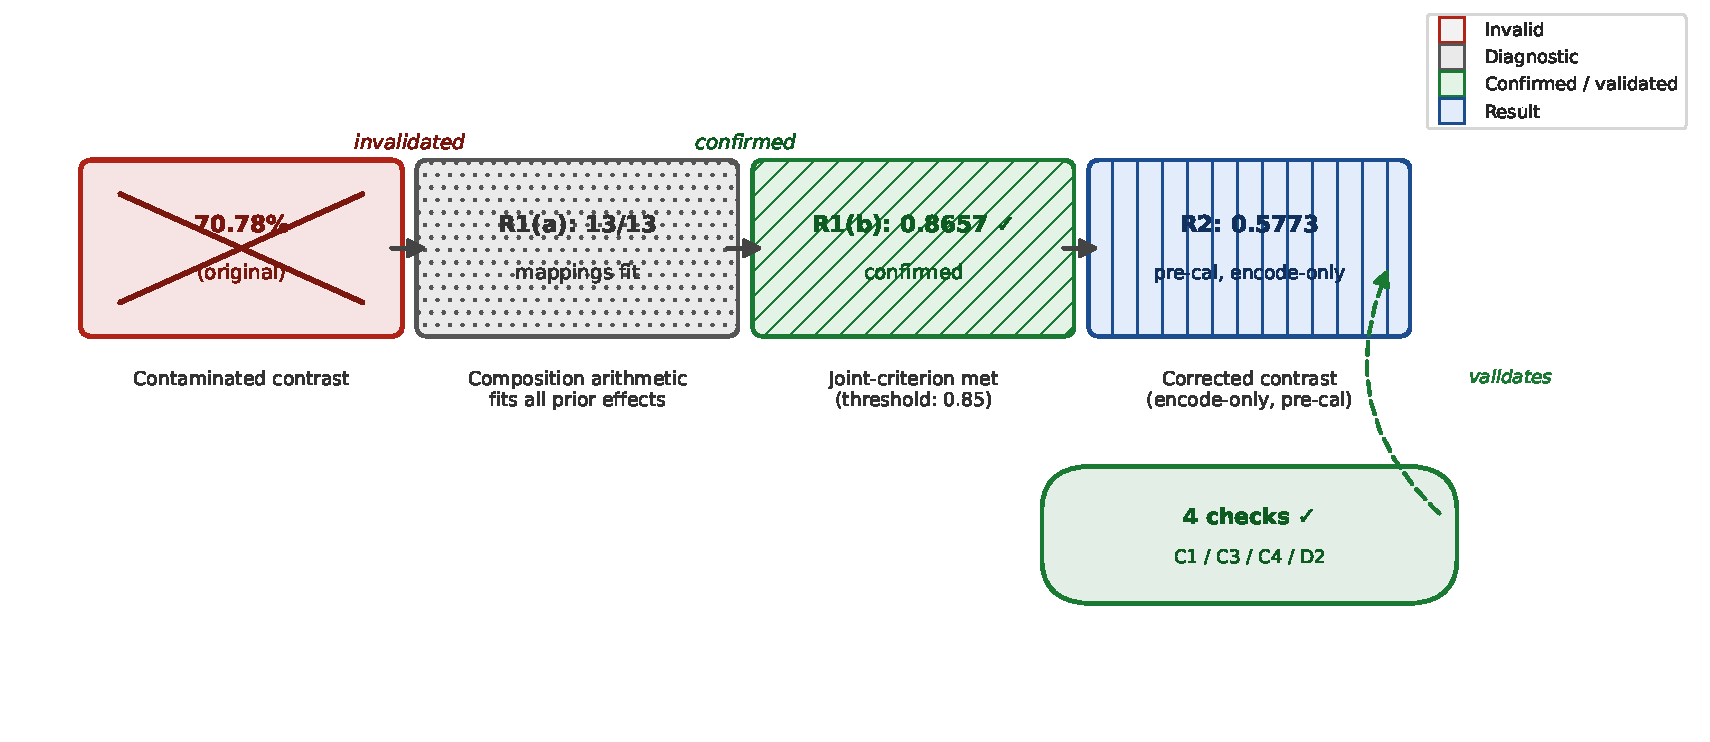
\includegraphics[width=\linewidth]{figures/fig1_discovery_timeline.pdf}
  \caption{Discovery-sequence timeline from the original contaminated contrast through diagnosis, confirmation, and validation. The original analysis reported 70.78\% balanced accuracy, invalidated once its class label was found to conflate four marker types. A composition-arithmetic diagnostic fit 13 of 13 prior effects (R1(a)); a direct encode-vs-test decode reached 0.8657 $\pm$ 0.0005 balanced accuracy against a pre-registered 0.85 threshold (R1(b)), confirming the account. The corrected contrast (R2) yields a pre-calibration balanced accuracy of 0.5773 $\pm$ 0.0005, validated by four independent checks (C1/C3/C4/D2; see Supplementary Table S1).}
  \label{fig:1}
\end{figure}

\subsection{Composition diagnosis (R1(a))}\label{sec:r1a}

Before proposing any alternative account of what the pipeline's earlier results had actually been measuring, we tested whether the real per-subject, per-block composition of each pseudo- or real-class construction used in the analyses preceding this correction (computed directly from marker indices, with no classifier training involved) predicts that construction's previously reported classifier accuracy. Applied to every checked contrast in the "temporal drift"/rest-break-discontinuity investigation this paper withdraws, this composition-arithmetic diagnostic's predictions matched the historically reported effect in 13 of 13 cases: 12 in both direction and magnitude, and one (the early/late contrast's exact cross-script magnitude) in direction only, a discrepancy we flag as noted rather than treat as a forced fit. This diagnostic step is arithmetic, not confirmatory on its own; it establishes that a composition-based account is consistent with the entire prior evidence base, which motivates but does not by itself decide the joint-criterion decode reported next.

\subsection{Joint-criterion confirmation (R1(b))}\label{sec:r1b}

We then re-epoched the dataset preserving all eight original marker codes as distinct classes and directly decoded encode-phase identity against test-phase identity \cite{pallerkutas1992,curran2000}, evaluating the result against the pre-registered joint criterion described in \S\ref{sec:dataset}: the composition-arithmetic diagnosis (\S\ref{sec:r1a}) together with a direct decode exceeding 0.85 balanced accuracy after calibration. This direct decode reached 0.8657 $\pm$ 0.0005 balanced accuracy, clearing the pre-registered threshold. \textbf{With both halves of the joint criterion satisfied, the unified composition explanation is confirmed in full, and the drift/rest-break-discontinuity mechanistic account previously proposed is formally withdrawn.} This closes out, rather than merely supersedes, the withdrawn account's full evidentiary basis: the composition account subsumes what that account had been built to explain, and we do not individually re-litigate each withdrawn finding in what follows (see \S\ref{sec:discussion} for the drift/rest-break investigation's place in this paper's argument).

\subsection{The corrected contrast (R2)}\label{sec:r2}

Restricting to encode-phase trial onsets only, the one epoch class carrying an unambiguous, uncontaminated, one-per-behavioral-trial Search/Memorize label (\S\ref{sec:dataset}), yields a pre-calibration balanced accuracy of 0.5773 $\pm$ 0.0005, 7.73 $\pm$ 0.05 percentage points above a chance floor near 50\%, the first Search-vs-Memorize, cross-subject, pre-calibration result reported in this paper that is not at chance. The corresponding post-calibration balanced accuracy is 0.7311 $\pm$ 0.0005. \textbf{We state explicitly, on this first mention and not as a trailing qualification, that this post-calibration figure has not itself been tested by any of the four validation controls reported in \S\ref{sec:validation}: all four controls in this paper test only the pre-calibration axis of R2's result, and the post-calibration figure inherits none of that validation}, a limitation we return to in full in \S\ref{sec:limitations}, not merely flagged in passing here.

For reference, R1(b)'s own encode-vs-test decode (\S\ref{sec:r1b}) reached a pre-calibration balanced accuracy of 0.8121 $\pm$ 0.0005 and a post-calibration balanced accuracy of 0.8657 $\pm$ 0.0005, with an AUC of 0.9276 pre-calibration and 0.9533 post-calibration, substantially higher than R2's corresponding pre-calibration figure (0.5773 $\pm$ 0.0005) throughout, as expected for a decode of phase identity (encode vs. test) rather than a within-phase task-instruction decode.

A third contrast (R3) retains the original 200-epoch-per-class construction described in \S\ref{sec:dataset} but drops the 75 New-Lure epochs per class per subject, recognition-test responses to items studied under neither task condition, leaving 125 epochs per class per subject (50 encode onsets, 50 test-target responses, 25 test-distractor responses). Its purpose is to quantify how much of the original 70.78\% headline (\S\ref{sec:headline}) was contributed specifically by New-Lure epochs, which by construction carry no encoding-condition information at all. R3 yields a pre-calibration balanced accuracy of 0.5293 $\pm$ 0.0005 and a post-calibration balanced accuracy of 0.7186 $\pm$ 0.0005. It is descriptive rather than pass/fail (no criterion was pre-registered for it), and we report it here as a composition-gradient benchmark alongside R1(b) and R2, not as a novel finding in its own right.

R2's pre-calibration result (0.5773 $\pm$ 0.0005) is the corrected contrast's central claim carried forward through the rest of this paper. Before treating it as established, we subjected it to four independent validation controls, reported next in \S\ref{sec:validation}.

\subsection{Validation controls}\label{sec:validation}

We report the four robustness checks applied to R2's pre-calibration result (0.5773 $\pm$ 0.0005) as their own subsection, separate from the evidence line above, because each of them tests that already-reported result rather than contributing a new finding of its own: presenting them as additional entries in a flat evidence list would overstate how much independent evidence this paper actually contains.

\subsubsection{C1: Shuffled-label null on the exact R2 dataset}

We computed 30 within-subject label shuffles on the exact R2 dataset (not a null reused from a differently-composed prior contrast) using the identical calibrated LOSO pipeline, per standard permutation-testing practice \cite{nicholsholmes2002}. The resulting null distribution has mean 0.4990 and SD 0.0103 $\pm$ 0.0001; R2's real value (0.5773 $\pm$ 0.0005) falls outside the 95\% confidence interval by both the percentile and normal-approximation method. Per the pre-registered rule, this is a genuine, subject-generalizable signal, not an artifact of this particular null construction.

\subsubsection{C3: Leave-one-subject-out jackknife}

To test whether R2's result is carried by one or two influential subjects rather than distributed across the cohort, we recomputed the 29-fold mean with each subject excluded in turn. The resulting leave-one-out means range from 0.5703 $\pm$ 0.0005 to 0.5852 $\pm$ 0.0005; every one of the 29 exclusions leaves the mean well above the pre-registered null-CI threshold of 0.5172 $\pm$ 0.0005, and no single exclusion shifts the mean by more than 0.0079 $\pm$ 0.0005 (the largest shift, from excluding sub-03), far short of the 0.0301 $\pm$ 0.0005 threshold pre-registered to flag an individually influential fold. R2's result is not carried by any single subject (see Supplementary Table S1).

\begin{figure}[htbp]
  \centering
  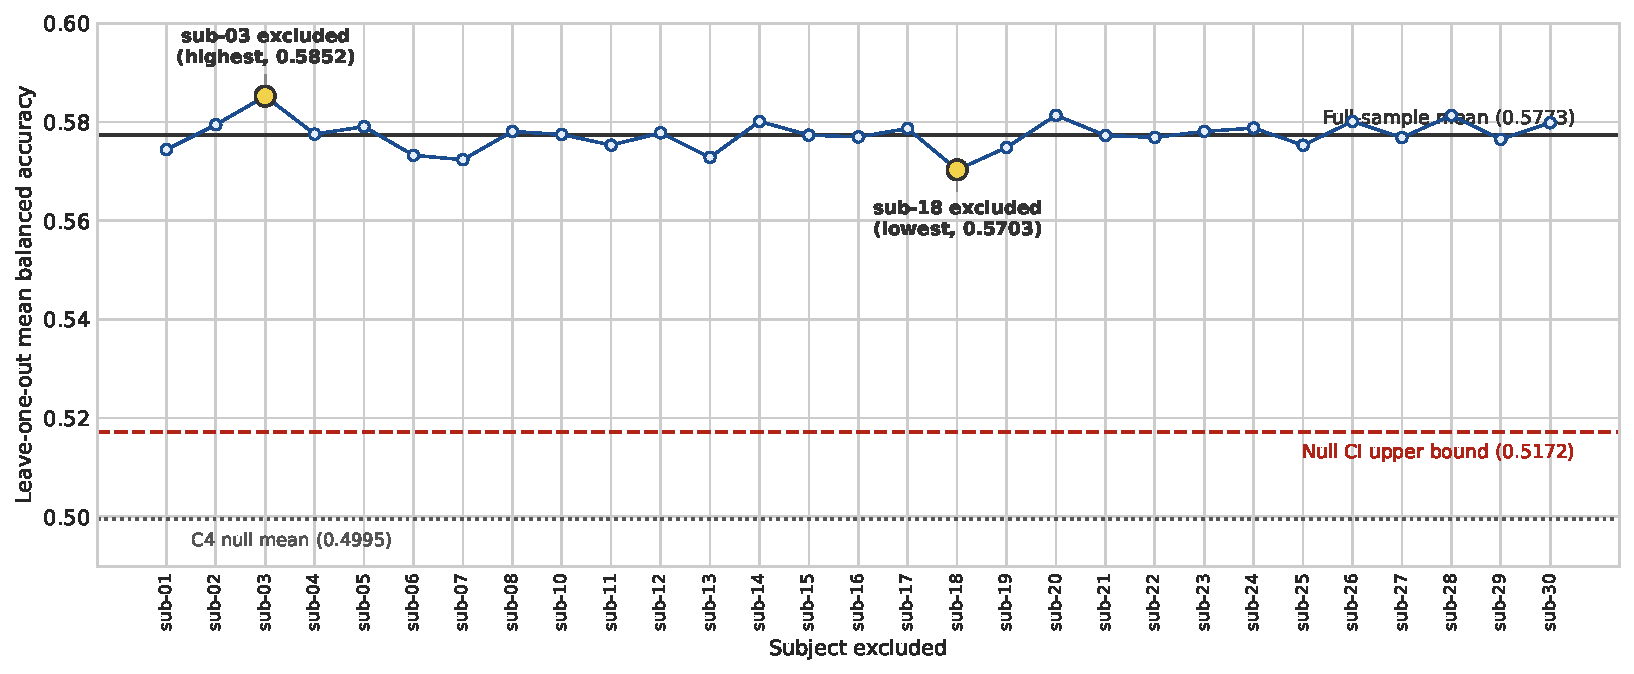
\includegraphics[width=\linewidth]{figures/fig2_c3_jackknife.pdf}
  \caption{Leave-one-subject-out jackknife: the 29 leave-one-out mean pre-calibration balanced accuracies obtained by excluding each subject from R2 in turn (see Supplementary Table S1). Reference lines mark the full-sample mean (0.5773 $\pm$ 0.0005), the null 95\% CI upper bound (0.5172 $\pm$ 0.0005), and the C4 null mean (0.4995). No exclusion drops the mean below the null CI upper bound; the extremes are sub-03 (highest, 0.5852 $\pm$ 0.0005) and sub-18 (lowest, 0.5703 $\pm$ 0.0005).}
  \label{fig:2}
\end{figure}

\subsubsection{C4: Higher-resolution shuffled-label null}

To sharpen C1's p-value estimate, we repeated the shuffled-label procedure at 500 shuffles rather than 30, using the same base seed so that the first 30 of the 500 shuffles reproduced C1's original 30 values exactly in the run reported here; on re-execution this check is subject to the same single-trial movement described in \S\ref{sec:data}, and its verdict is unchanged under the tolerance applied throughout. The 500-shuffle null has mean 0.4995 and SD 0.0112, with a 95\% confidence interval of [0.4764 $\pm$ 0.0005, 0.5199 $\pm$ 0.0005] (percentile) or [0.4776, 0.5214] (normal-approximation); both exclude R2's real value (0.5773 $\pm$ 0.0005) on the same side as C1's coarser-resolution interval, satisfying the pre-registered consistency rule. At this resolution, the empirical p-value is p = 0 by the raw convention (0 of 500 shuffles at or above R2's real value) and p $<$ 0.002 by the add-one-corrected convention.

\begin{figure}[htbp]
  \centering
  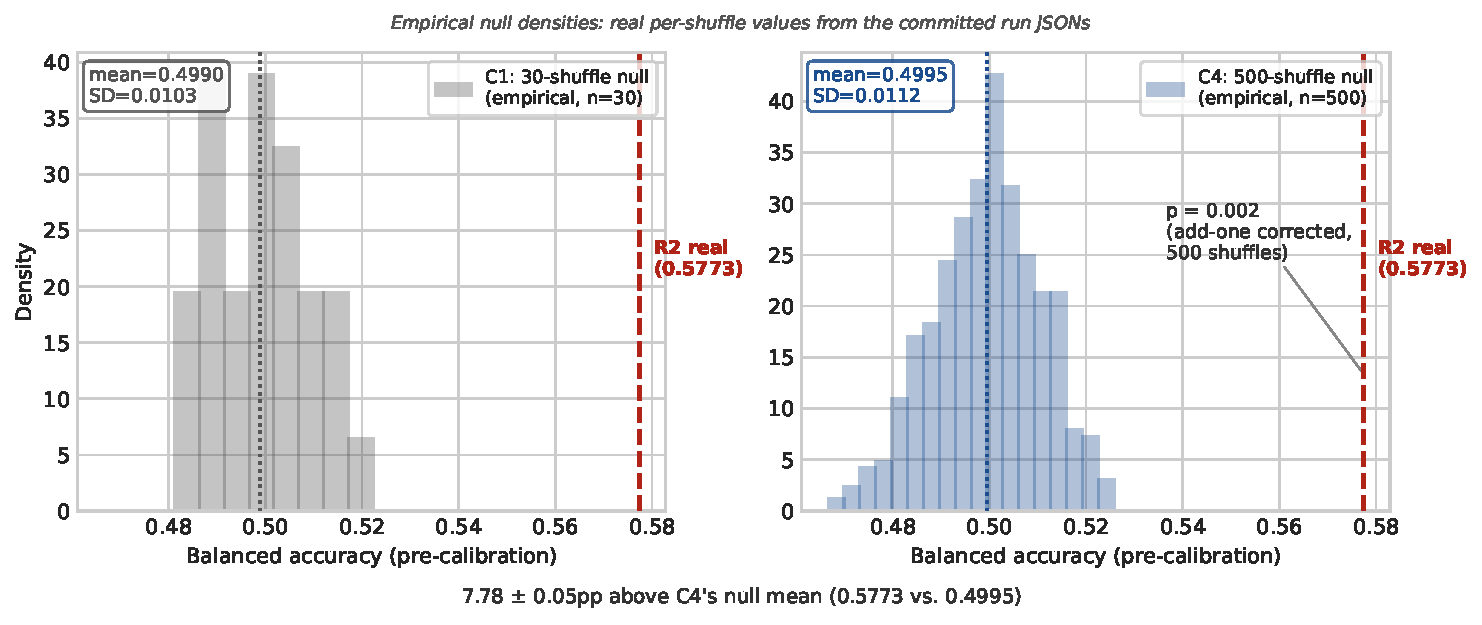
\includegraphics[width=\linewidth]{figures/fig3_null_distribution.pdf}
  \caption{R2's pre-calibration balanced accuracy (0.5773 $\pm$ 0.0005) against two shuffled-label null distributions computed on the exact R2 dataset: C1 (30 shuffles, mean 0.4990, SD 0.0103 $\pm$ 0.0001) and C4 (500 shuffles, mean 0.4995, SD 0.0112, p $<$ 0.002 add-one-corrected). Null densities are the real per-shuffle values from each control's own committed run record. R2 falls 7.78 $\pm$ 0.05 percentage points above C4's null mean, the higher-resolution and thus preferred baseline of the two.}
  \label{fig:3}
\end{figure}

\subsubsection{D2: Parity-split replication}

The final check addresses whether R2's signal could instead reflect block-order or session-position rather than task instruction specifically, the question a counterbalanced design is meant to guard against \cite{greenwald1976}. Two distinct arguments bear on this question, and we keep them separate because they come from different sources and are not the same evidence.

The first argument follows from R2's own pooled design (\S\ref{sec:dataset}), not from any additional analysis: because odd-numbered subjects complete Search first and even-numbered subjects complete Memorize first, the two subgroups' position-to-label mappings are inversely opposed within R2's single pooled 29-fold training pool. A classifier relying purely on session position, rather than task instruction, would be trained on directly contradictory position-to-label signal across the two subgroups and would be expected to degrade toward chance, not to reach R2's actual result of 0.5773 $\pm$ 0.0005. This argument requires no further data; it follows from R2's counterbalanced design as described in \S\ref{sec:dataset}.

The second argument is D2 itself: we split R2's 29 subjects into their two parity-defined subgroups and re-ran the calibrated LOSO pipeline within each subgroup separately, each tested against its own freshly-computed within-group shuffled-label null (a pooled null would be too tight to be valid at this smaller per-group sample size). The odd-numbered, Search-first subgroup (n=14) reached a pre-calibration balanced accuracy of 0.6157 $\pm$ 0.001 against its own within-group null (mean 0.4987, 95\% CI [0.4793 $\pm$ 0.0005, 0.5179 $\pm$ 0.0005]), outside the CI. The even-numbered, Memorize-first subgroup (n=15) reached 0.5582 $\pm$ 0.001 against its own null (mean 0.4985, 95\% CI [0.4724 $\pm$ 0.0005, 0.5223 $\pm$ 0.0005]), also outside the CI. Both subgroups individually clear their own within-group null. D2's contribution is this robustness result, the signal survives being re-tested separately, at smaller sample size, within each subgroup, not the inversely-mapped-position argument above, which belongs to R2's pooled design and not to D2.

We note directly here, as an observed fact rather than a resolved one, that the two subgroups' gaps above their own nulls' means are not equal: the odd subgroup's gap above its null's mean (0.6157 $-$ 0.4987 = 0.1170 $\pm$ 0.001) is roughly twice the even subgroup's gap above its null's mean (0.5582 $-$ 0.4985 = 0.0597 $\pm$ 0.001). Both gaps are individually significant and both subgroups clear their own CI, so this asymmetry does not contradict D2's verdict above, but it is a real feature of the result that we do not explain here, and we return to it in \S\ref{sec:limitations}.

\begin{figure}[htbp]
  \centering
  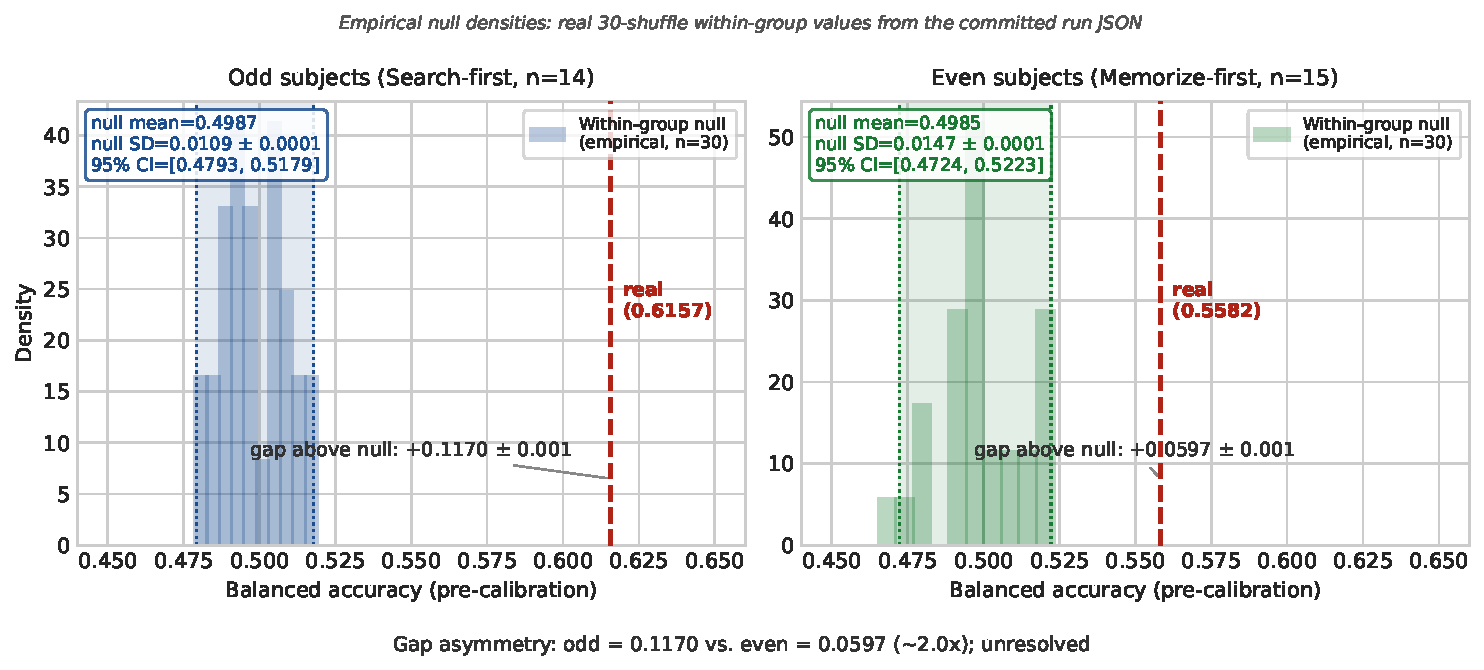
\includegraphics[width=\linewidth]{figures/fig4_d2_parity_split.pdf}
  \caption{D2 parity-split replication: pre-calibration balanced accuracy for odd (Search-first, n=14, 0.6157 $\pm$ 0.001) and even (Memorize-first, n=15, 0.5582 $\pm$ 0.001) subject subgroups against each subgroup's own within-group shuffled-label null (empirical, the real 30 per-shuffle values from each subgroup's own committed run record). Both subgroups clear their own 95\% CI. The gap above each subgroup's null mean is asymmetric: 0.1170 $\pm$ 0.001 (odd) vs. 0.0597 $\pm$ 0.001 (even), roughly 2$\times$, unresolved (\S\ref{sec:limitations}).}
  \label{fig:4}
\end{figure}

Taken together, these four checks establish that R2's pre-calibration result (0.5773 $\pm$ 0.0005) is a real, subject-generalizable signal (distinguishable from a shuffled-label null at two resolutions, not attributable to any single subject, and not explained by block-order or session-position alone), but they do not establish the validity of R2's post-calibration result (\S\ref{sec:r2}), which none of the four checks tested, or a mechanism for the signal beyond ruling out the specific alternatives each was designed to test, both of which we take up in \S\ref{sec:limitations}.

\section{A Reusable Diagnostic Protocol}\label{sec:protocol}

The corrections described in \S\ref{sec:methods} and \S\ref{sec:results} generalize beyond this dataset to any blocked, multi-phase paradigm with a hand-written marker/event dictionary. We summarize them here as a four-step checklist for a practitioner encountering a similar design, independent of this paper's own results.

\begin{enumerate}
\item \textbf{Compute real per-subject class composition from raw markers.} Before trusting any classifier result in a multi-phase design, compute each class label's exact per-subject composition directly from marker indices and check it against the dictionary's stated definition. This requires no classifier training and can rule a labeling confound in or out before any model is fit, the central diagnostic in this protocol.
\item \textbf{Require a joint criterion before declaring a confound confirmed.} Composition arithmetic alone is suggestive, not decisive. Pair it with a direct classifier decode of the identified confound, evaluated against a pre-registered accuracy threshold, before treating the account as confirmed.
\item \textbf{Validate any corrected contrast against a null computed on the exact corrected dataset.} A null built from a differently-composed prior contrast is not a valid reference; re-derive it from the corrected data itself, at whatever resolution the claim requires.
\item \textbf{Test the corrected contrast against its own structural counterbalancing.} If the corrected design still permits a confound the paradigm's own counterbalancing could resolve (e.g., block order), test it directly within each counterbalanced subgroup, against that subgroup's own null, rather than assuming the pooled result already rules it out.
\end{enumerate}

Pair every step above with the reporting discipline followed throughout this paper: pre-calibration accuracy alongside any calibrated figure, and class-balance/majority-rate/balanced-accuracy hardening on every classification result.

\section{Limitations}\label{sec:limitations}

Six limitations qualify the result reported in \S\ref{sec:results} and \S\ref{sec:validation}. We state all six in full, not in an abbreviated form: the finding being positive rather than null does not reduce how many open questions remain around it.

\begin{enumerate}
\item \textbf{Post-calibration validity is untested.} All four checks in \S\ref{sec:validation} (C1, C3, C4, D2) test only the pre-calibration axis of R2's result. Not one of them says anything about R2's post-calibration figure (0.7311 $\pm$ 0.0005, \S\ref{sec:r2}): C1 and C4's shuffled-label nulls are computed against pre-calibration accuracy; C3's jackknife is computed over pre-calibration fold values; D2's within-group replication is likewise restricted to the pre-calibration axis. The post-calibration figure inherits none of the validation established for the pre-calibration figure. The finding established in \S\ref{sec:calibration} that post-calibration accuracy is a few-shot subject-adaptive result \cite{he2020,jayaram2016}, not a subject-independent one, applies to R2's post-calibration number exactly as it applied to every post-calibration number reported earlier in this paper. A reader who takes 0.7311 $\pm$ 0.0005 as validated in the way 0.5773 $\pm$ 0.0005 is validated would be extending this paper's evidence further than \S\ref{sec:validation} actually supports.
\item \textbf{Task-instruction vs. other encoding-phase differences is substantially, but not completely, addressed.} D2 (\S\ref{sec:validation}) rules out a simple session-position confound: because Search and Memorize occupy opposite positions across the two parity subgroups, a pure position effect could not by itself produce the same-direction elevation D2 observes in both subgroups. This narrows the space of alternative explanations but does not close it. D2 tests one specific alternative (session position) against one specific rival (task instruction); it does not rule out every possible non-task-instruction explanation. Per-subject stimulus-set identity, for instance, remains confounded with class within each subject by the paradigm's own design, and no control in this paper isolates that factor specifically. The mechanism behind R2's signal is narrowed by D2, not fully isolated.
\item \textbf{D2's parity-group effect-size asymmetry is unexplained.} The odd-numbered subgroup's gap above its own null's mean (0.1170 $\pm$ 0.001) is roughly twice the even-numbered subgroup's gap (0.0597 $\pm$ 0.001, \S\ref{sec:validation}). We record this here as an observed fact with no available explanation, not as evidence against D2's verdict, since both subgroups individually clear their own null and the asymmetry does not change that, and not as a minor variance note to be waved past, since a roughly two-fold difference in effect size between two subgroups of an otherwise-validated result is exactly the kind of asymmetry that would matter if it turned out to have a real cause (a genuine difference in decodability between Search-first and Memorize-first subjects, for instance) rather than being small-sample variation at n=14/15. We do not pursue a further dedicated control to distinguish these possibilities, given the group sizes involved, and record the asymmetry here as open rather than resolved in either direction.
\item \textbf{The effect size is modest in absolute terms.} R2's pre-calibration elevation is 7.73 $\pm$ 0.05 percentage points above a chance floor near 50\% (\S\ref{sec:r2}, \S\ref{sec:validation}). This is a factual description of the result's practical magnitude, not a hedge on its validity: the signal is real and subject-generalizable (\S\ref{sec:validation}), and its modest size is a property of what was found, stated here at the same register as it is stated in the Abstract, not diminished by appearing in a Limitations section.
\item \textbf{Single-seed basis.} Every evaluation in this paper, R1(b), R2, R3, and all four controls in \S\ref{sec:validation}, uses a single fixed seed (seed = 42, \S\ref{sec:calibration}) rather than a multi-seed protocol. This is a deliberate, disclosed cost tradeoff, not an oversight, and matches the convention used throughout the analyses preceding this correction; seed-to-seed variance in any of this paper's reported numbers has not been characterized.
\item \textbf{Alignment-scheme dependency.} All results in this paper use the pooled-subject form of Euclidean Alignment described in \S\ref{sec:calibration}, a single alignment transform computed from the training pool and applied uniformly, not a parametrized per-subject or Riemannian-mean module. This pipeline choice is unchanged from before this correction and has not been re-tested under an alternative alignment scheme for the corrected contrast described here.
\end{enumerate}

\section{Discussion}\label{sec:discussion}

This paper began as an investigation into a null result and the artifact that produced it, and ends as a report of a real, modest, validated signal that a labeling error had hidden. We state this shift directly rather than leaving it for the reader to infer from the ordering of \S\ref{sec:results}: the central claim of this paper is not that Search-vs-Memorize decoding is undetectable in this dataset, but that it is detectable, once its class labels are corrected, at a magnitude far more modest than the original headline number (\S\ref{sec:headline}) suggested.

The diagnostic protocol described in \S\ref{sec:protocol} is, in this paper, in service of recovering a signal rather than debunking one, the opposite direction from how a similar composition-based argument was originally used in the withdrawn drift investigation described in this paper. The underlying method (composition arithmetic against raw markers, a joint criterion before confirming any account, and null validation on the exact corrected dataset) is agnostic to which direction the correction points. It would apply identically to a design where correcting a marker-dictionary error revealed a null where a spurious effect had previously been reported, the reverse of what happened here.

The withdrawn drift/rest-break-discontinuity account (\S\ref{sec:r1b}) was not wasted effort. It correctly established that the original, contaminated contrast's calibrated accuracy was not diagnostic of task content; that finding stands, unchanged by anything in this paper. What has changed is the explanation for \emph{why}: it is R1(b)'s composition account (\S\ref{sec:r1b}), not a flaw in the drift investigation's own logic, that explains why the original contrast behaved the way it did. The drift account is withdrawn as an explanation for a contrast that no longer appears anywhere in this paper's argument, not refuted on its own terms.

Three things this paper does not claim, stated explicitly. First, it does not critique ds005189 or its original authors' own published work (\S\ref{sec:dataset}): the labeling error described here belongs entirely to our own analysis pipeline, not to the dataset or its collection. Second, the 7.73 $\pm$ 0.05 percentage-point effect reported in \S\ref{sec:r2} and \S\ref{sec:limitations} is not claimed to be large in absolute terms; it is real and subject-generalizable, at the modest magnitude stated. Third, the task-instruction-vs-position question is not claimed to be fully closed: D2 (\S\ref{sec:validation}) rules out a simple position confound, but the parity-group effect-size asymmetry it also revealed remains unresolved (\S\ref{sec:limitations}), and we do not treat D2 as having settled the broader question of what drives R2's signal.

\section{Conclusion}\label{sec:conclusion}

This paper reports three things in sequence. First, a label-dictionary error in our own analysis pipeline (a class definition built from four structurally distinct marker types rather than one) produced a 70.78\% headline number that was arithmetically correct and scientifically uninterpretable as a claim about Search-vs-Memorize decoding (\S\ref{sec:headline} and \S\ref{sec:invalidation}). Second, a composition-arithmetic diagnostic paired with a direct joint-criterion decode (\S\ref{sec:r1a} and \S\ref{sec:r1b}) together confirmed the error's explanation in full and formally withdrew the drift/rest-break-discontinuity account previously proposed for the same contrast. Third, correcting the contrast to encode-phase trials only recovers a real, cross-subject, pre-calibration signal (0.5773 $\pm$ 0.0005) that four independent checks, a shuffled-label null at two resolutions (C1, C4), a leave-one-subject-out jackknife (C3), and a parity-split replication (D2) (\S\ref{sec:validation}), establish as genuine and not attributable to any single subject or to session position alone, while leaving its post-calibration validity and full mechanism open (\S\ref{sec:limitations}). Beyond this dataset, the paper's contribution is the diagnostic protocol itself (\S\ref{sec:protocol}): composition arithmetic against raw markers, a joint criterion before confirming any account, and null validation on the exact corrected dataset apply to any blocked, multi-phase paradigm with a hand-written event dictionary, independent of whether the correction it prompts reveals a null or, as here, recovers a signal that a labeling error had hidden.

\section{Data and Code Availability}\label{sec:data}

\begin{sloppypar}\textbf{Dataset.} ds005189 (OpenNeuro accession ds005189), DOI \url{https://doi.org/10.18112/openneuro.ds005189.v1.0.1} \cite{markiewicz2021,gorgolewski2016}, license CC0.\end{sloppypar}

\textbf{Code.} All scripts referenced in this paper, R1(a), R1(b)/R2/R3, C1, C3, C4, D2, and the D1 transcription utility, together with \texttt{results/RESULTS\_LEDGER.md} and \texttt{DECISIONS.md}, are available at \url{https://github.com/HassanSidd0946/Search-vs-Memorize-Correction}. Commit hash: 4082949c; a specific commit will be tagged at submission.

\textbf{Reproducibility.} The classification pipeline underlying every result in this paper is not bit-exactly reproducible across re-runs on different compute hardware: unpinned BLAS/LAPACK thread-count racing and OpenBLAS's runtime microarchitecture dispatch can each shift a small number of individual fold-level classifications between otherwise-identical runs. Every balanced accuracy, AUC, and derived threshold reported in this paper is therefore cited with an explicit tolerance (typically $\pm$0.0005) reflecting the largest such single-trial movement observed for that quantity, rather than as a bare point estimate. This reproducibility claim is scoped specifically to the modelling layer: the epoching layer that produces this pipeline's input is cached per subject on first computation and reused across analyses. Subject 01's checkpoint is re-validated against its expected post-exclusion marker counts on every pipeline execution and automatically rebuilt from raw if stale; the composition-level scripts additionally assert the expected total sample count at load time. Count-based validation of this kind cannot detect floating-point drift in the 1--40 Hz band-pass filter or 250 Hz resampling step that produce the underlying epoched signal (\S\ref{sec:calibration}), and the same cross-host dispatch non-determinism that affects the modelling layer could in principle affect these operations too; the epoching layer has not been independently re-derived from raw since its original run, so its own run-to-run numerical stability is unmeasured, and the reproducibility claim above does not extend to it.

\textbf{Pre-registration record.} Every verdict threshold applied in \S\ref{sec:results} and \S\ref{sec:validation} traces to a dated entry in \texttt{DECISIONS.md}, recorded before the corresponding analysis was run.

\textbf{Ethics.} This paper conducts no new data collection. The re-analysis reported here is covered by the source dataset's existing approval (Ethics committee, Faculty of Psychology and Sports Sciences, Goethe University Frankfurt, approval ID 2014-106R1). Re-analysis of CC0-licensed data does not require separate approval; conformance with journal policy should be confirmed at submission.

\textbf{Funding.} This research received no specific grant from any funding agency in the public, commercial, or not-for-profit sectors.

\textbf{Declaration of competing interest.} The authors declare no competing financial interests or personal relationships that could have appeared to influence the work reported in this paper.

\textbf{CRediT authorship contribution statement.} Muhammad Hassan Siddiqui: Conceptualization, Methodology, Software, Formal analysis, Writing - original draft. Muhammad Adil Usmani: Validation, Writing - review \& editing.

\bibliographystyle{elsarticle-num}
\bibliography{references}

\clearpage
\section*{Supplementary Material}
Supplementary Table~S1, referenced throughout \S\ref{sec:validation}, appears at the end of this document.

\begin{table}[!p]
\caption{Supplementary Table~S1. Leave-one-subject-out (LOO) jackknife analysis of R2 pre-calibration balanced accuracy (C3). Full-sample mean $= 0.5773 \pm 0.0005$. No single exclusion drops the LOO mean below the pre-registered null CI upper bound ($ 0.5172 \pm 0.0005$).}
\label{tab:s1}
\centering
\begin{tabular}{lccc}
\toprule
Subject excluded & Per-fold accuracy & LOO mean & Shift from full-sample mean \\
\midrule
sub-01 & 0.6600 $\pm$ 0.012 & 0.5744 $\pm$ 0.0005 & -0.0030 $\pm$ 0.0005 \\
sub-02 & 0.5188 $\pm$ 0.012 & 0.5794 $\pm$ 0.0005 & +0.0021 $\pm$ 0.0005 \\
sub-03 & 0.3571 $\pm$ 0.012 & 0.5852 $\pm$ 0.0005 & +0.0079 $\pm$ 0.0005 \\
sub-04 & 0.5720 $\pm$ 0.012 & 0.5775 $\pm$ 0.0005 & +0.0002 $\pm$ 0.0005 \\
sub-05 & 0.5296 $\pm$ 0.012 & 0.5790 $\pm$ 0.0005 & +0.0017 $\pm$ 0.0005 \\
sub-06 & 0.6921 $\pm$ 0.012 & 0.5732 $\pm$ 0.0005 & -0.0041 $\pm$ 0.0005 \\
sub-07 & 0.7173 $\pm$ 0.012 & 0.5723 $\pm$ 0.0005 & -0.0050 $\pm$ 0.0005 \\
sub-08 & 0.5570 $\pm$ 0.012 & 0.5781 $\pm$ 0.0005 & +0.0007 $\pm$ 0.0005 \\
sub-10 & 0.5739 $\pm$ 0.012 & 0.5775 $\pm$ 0.0005 & +0.0001 $\pm$ 0.0005 \\
sub-11 & 0.6346 $\pm$ 0.012 & 0.5753 $\pm$ 0.0005 & -0.0020 $\pm$ 0.0005 \\
sub-12 & 0.5651 $\pm$ 0.012 & 0.5778 $\pm$ 0.0005 & +0.0004 $\pm$ 0.0005 \\
sub-13 & 0.7040 $\pm$ 0.012 & 0.5728 $\pm$ 0.0005 & -0.0045 $\pm$ 0.0005 \\
sub-14 & 0.5000 $\pm$ 0.012 & 0.5801 $\pm$ 0.0005 & +0.0028 $\pm$ 0.0005 \\
sub-15 & 0.5778 $\pm$ 0.012 & 0.5773 $\pm$ 0.0005 & 0.0000 $\pm$ 0.0005 \\
sub-16 & 0.5880 $\pm$ 0.012 & 0.5770 $\pm$ 0.0005 & -0.0004 $\pm$ 0.0005 \\
sub-17 & 0.5404 $\pm$ 0.012 & 0.5787 $\pm$ 0.0005 & +0.0013 $\pm$ 0.0005 \\
sub-18 & 0.7746 $\pm$ 0.012 & 0.5703 $\pm$ 0.0005 & -0.0070 $\pm$ 0.0005 \\
sub-19 & 0.6476 $\pm$ 0.012 & 0.5748 $\pm$ 0.0005 & -0.0025 $\pm$ 0.0005 \\
sub-20 & 0.4654 $\pm$ 0.012 & 0.5813 $\pm$ 0.0005 & +0.0040 $\pm$ 0.0005 \\
sub-21 & 0.5797 $\pm$ 0.012 & 0.5773 $\pm$ 0.0005 & -0.0001 $\pm$ 0.0005 \\
sub-22 & 0.5905 $\pm$ 0.012 & 0.5769 $\pm$ 0.0005 & -0.0005 $\pm$ 0.0005 \\
sub-23 & 0.5568 $\pm$ 0.012 & 0.5781 $\pm$ 0.0005 & +0.0007 $\pm$ 0.0005 \\
sub-24 & 0.5377 $\pm$ 0.012 & 0.5788 $\pm$ 0.0005 & +0.0014 $\pm$ 0.0005 \\
sub-25 & 0.6351 $\pm$ 0.012 & 0.5753 $\pm$ 0.0005 & -0.0021 $\pm$ 0.0005 \\
sub-26 & 0.5000 $\pm$ 0.012 & 0.5801 $\pm$ 0.0005 & +0.0028 $\pm$ 0.0005 \\
sub-27 & 0.5916 $\pm$ 0.012 & 0.5768 $\pm$ 0.0005 & -0.0005 $\pm$ 0.0005 \\
sub-28 & 0.4665 $\pm$ 0.012 & 0.5813 $\pm$ 0.0005 & +0.0040 $\pm$ 0.0005 \\
sub-29 & 0.6016 $\pm$ 0.012 & 0.5765 $\pm$ 0.0005 & -0.0009 $\pm$ 0.0005 \\
sub-30 & 0.5078 $\pm$ 0.012 & 0.5798 $\pm$ 0.0005 & +0.0025 $\pm$ 0.0005 \\
\bottomrule
\end{tabular}
\end{table}

\end{document}
